\documentclass[aspectratio=169]{beamer}
%\usecolortheme{beaver}
\usepackage[english,ukrainian]{babel}
\usepackage{hyperref}
\hypersetup{colorlinks,urlcolor=blue}
\makeatletter
\DeclareUrlCommand\ULurl@@{%
  \def\UrlFont{\ttfamily\color{blue}}%
  \def\UrlLeft{\uline\bgroup}%
  \def\UrlRight{\egroup}}
\def\ULurl@#1{\hyper@linkurl{\ULurl@@{#1}}{#1}}
\DeclareRobustCommand*\ULurl{\hyper@normalise\ULurl@}
\makeatother
\usepackage[table]{colortbl}
\usecolortheme{whale}
\usepackage{etoolbox,refcount}
\usepackage{multicol}

\newcounter{countitems}
\newcounter{nextitemizecount}
\newcommand{\setupcountitems}{%
  \stepcounter{nextitemizecount}%
  \setcounter{countitems}{0}%
  \preto\item{\stepcounter{countitems}}%
}
\makeatletter
\newcommand{\computecountitems}{%
  \edef\@currentlabel{\number\c@countitems}%
  \label{countitems@\number\numexpr\value{nextitemizecount}-1\relax}%
}
\newcommand{\nextitemizecount}{%
  \getrefnumber{countitems@\number\c@nextitemizecount}%
}
\newcommand{\previtemizecount}{%
  \getrefnumber{countitems@\number\numexpr\value{nextitemizecount}-1\relax}%
}
\makeatother    
\newenvironment{AutoMultiColItemize}{%
\ifnumcomp{\nextitemizecount}{>}{3}{\begin{multicols}{2}}{}%
\setupcountitems\begin{itemize}}%
{\end{itemize}%
\unskip\computecountitems\ifnumcomp{\previtemizecount}{>}{3}{\end{multicols}}{}}
\usepackage[utf8]{inputenc}

\title{Прогнозування динаміки Індексу українських акцій (UX) за допомогою методів технічного аналізу та машинного навчання}
\author{Студент 4 курсу ОПП «Економічна кібернетика» Тараба В. С.\\ Науковий керівник: д. е. н., професор Ставицький А. В.}
\institute{Київський національний університет імені Тараса Шевченка\\Економічний факультет\\Кафедра економічної кібернетики}

\begin{document}
	
\begin{frame}
\titlepage
\end{frame}

\begin{frame}
\frametitle{План презентації}
\setbeamertemplate{section in toc}[circle]
%\setbeamercolor{section in toc}{fg=UniBlue}
%\setbeamercolor*{section in toc}{fg=UniBlue}
\tableofcontents
\end{frame}

\section{Опис дослідження та вхідних даних}

\begin{frame}
\frametitle{Опис дослідження}
\begin{itemize}
\item \alert {Метою дослідження}  є  аналіз  прибутковості  торгових  стратегій, що базуються  на  прогнозах  моделей  штучних  нейронних  мереж,  для  фондового індексу Індекс українських акцій (UX).
\tinyskip
\item \alert {Об’єктом дослідження} є Індекс українських акцій (UX).
\tinyskip
\item \alert {Предметом дослідження} є методи прогнозування фондових індексів та їх практичне застосування.
\tinyskip
\item \alert {Завданнями дослідження} є:
\begin{itemize}
    \item[\textcolor{orange}{\textbullet}] розглянути теоретичні засади аналізу фондового ринку, визначити основні методи, які використовуються для побудови прогнозу; розглянути основні методи технічного аналізу; 
    \item[\textcolor{orange}{\textbullet}] розглянути процес побудови  моделей машинного навчання та підбору оптимальних параметрів для моделі; підібрати відповідні моделі для індексу; 
    \item[\textcolor{orange}{\textbullet}] протестувати ефективність торгових стратегій, що базуються на сигналах підібраних  моделей та методах технічного аналізу, з врахуванням транзакційних витрат. 
\end{itemize}
\end{itemize}
\end{frame}

\begin{frame}
\frametitle{Оптимізаційний алгоритм}
\[ v_{t+1} = \beta_{1} v_{t} + (1-\beta_{1})\nabla J(W_{t}) \]\\
\[ cache_{t+1} = \beta_{2} cache_{t} + (1-\beta_{2})(\nabla J(W_{t}))^{2} \]\\
\[ W_{t+1} = W_{t}-\frac{\eta}{\sqrt{cache_{t+1}+\varepsilon}}v_{t+1} \]
\bigskip
\begin{itemize}
\item \alert {Оптимізаційний алгоритм Adam} є стандартним вибором для більшості нейронних мереж. Значення параметрів – за замовчуванням ($\eta$=0.001, $\beta_{1}$=0.9, $\beta_{1}$=0.999, $\varepsilon$=1e-07). 
\end{itemize}
\end{frame}

\section{Порівняння результатів торгових стратегій}

\begin{frame}
\frametitle{Результати торгових стратегій, які базуються на сигналах методів ТА}
\begin{center}
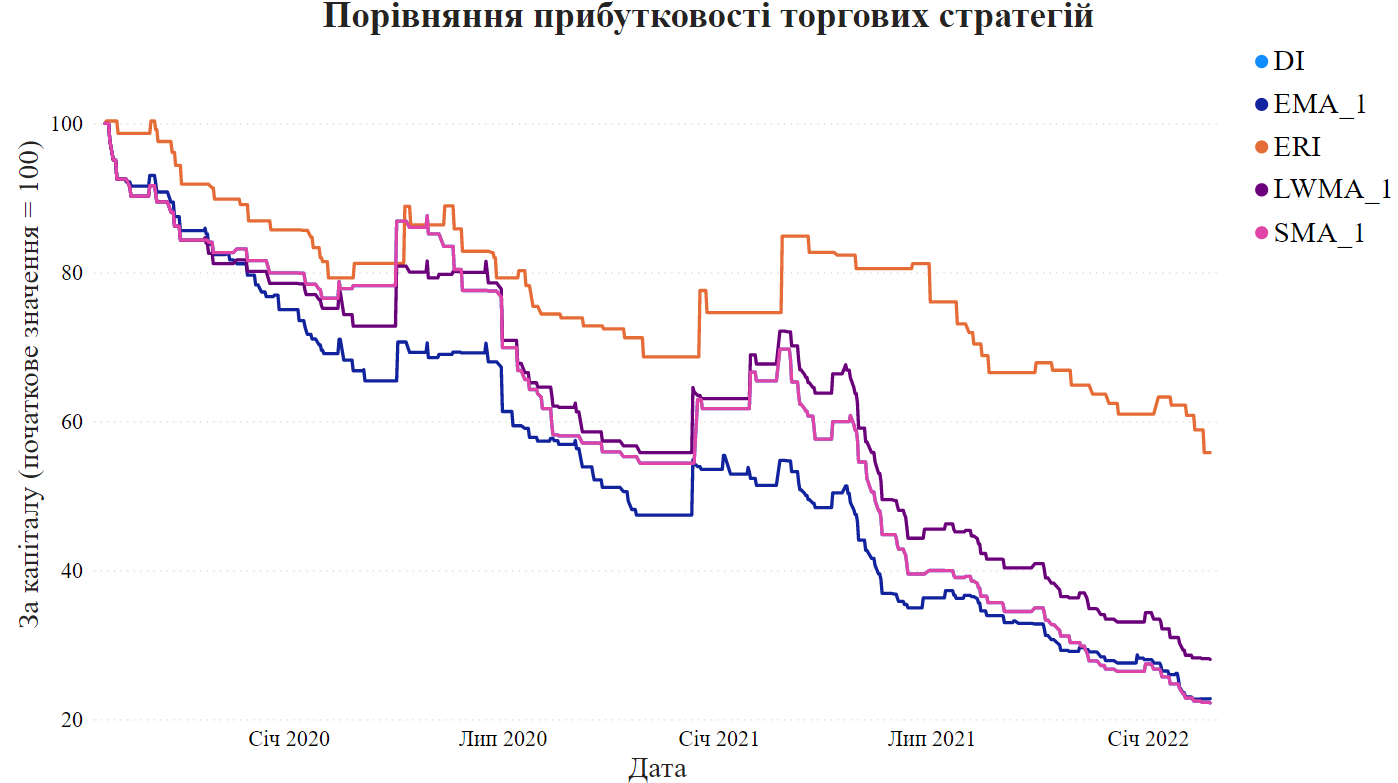
\includegraphics[scale=0.35]{Results Part 1.png}
\end{center}
\end{frame}

\begin{frame}
\frametitle{Результати торгових стратегій, які базуються на сигналах методів ТА}
\begin{center}
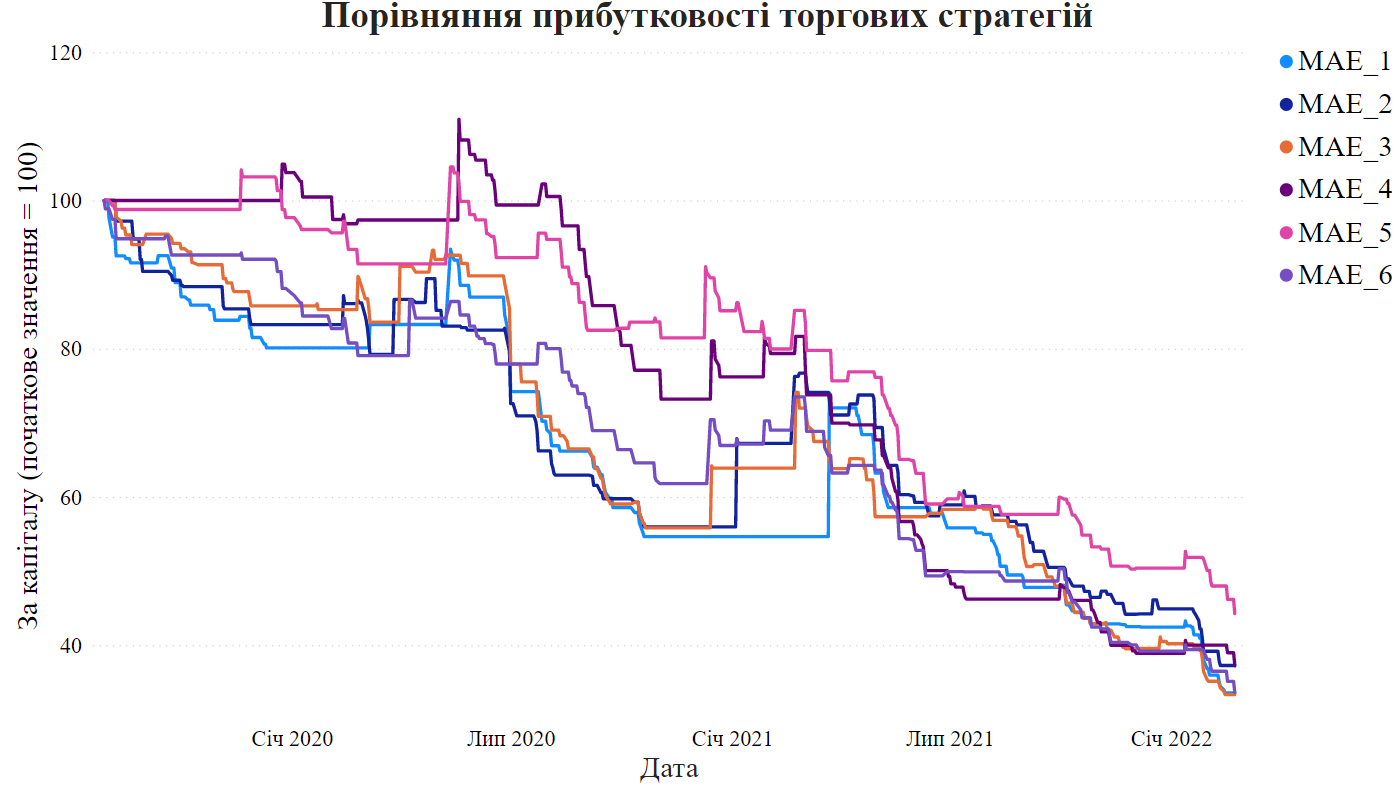
\includegraphics[scale=0.35]{Results Part 2.png}
\end{center}
\end{frame}

\begin{frame}
\frametitle{Результати торгових стратегій, які базуються на прогнозах методів машинного навчання}
\begin{center}
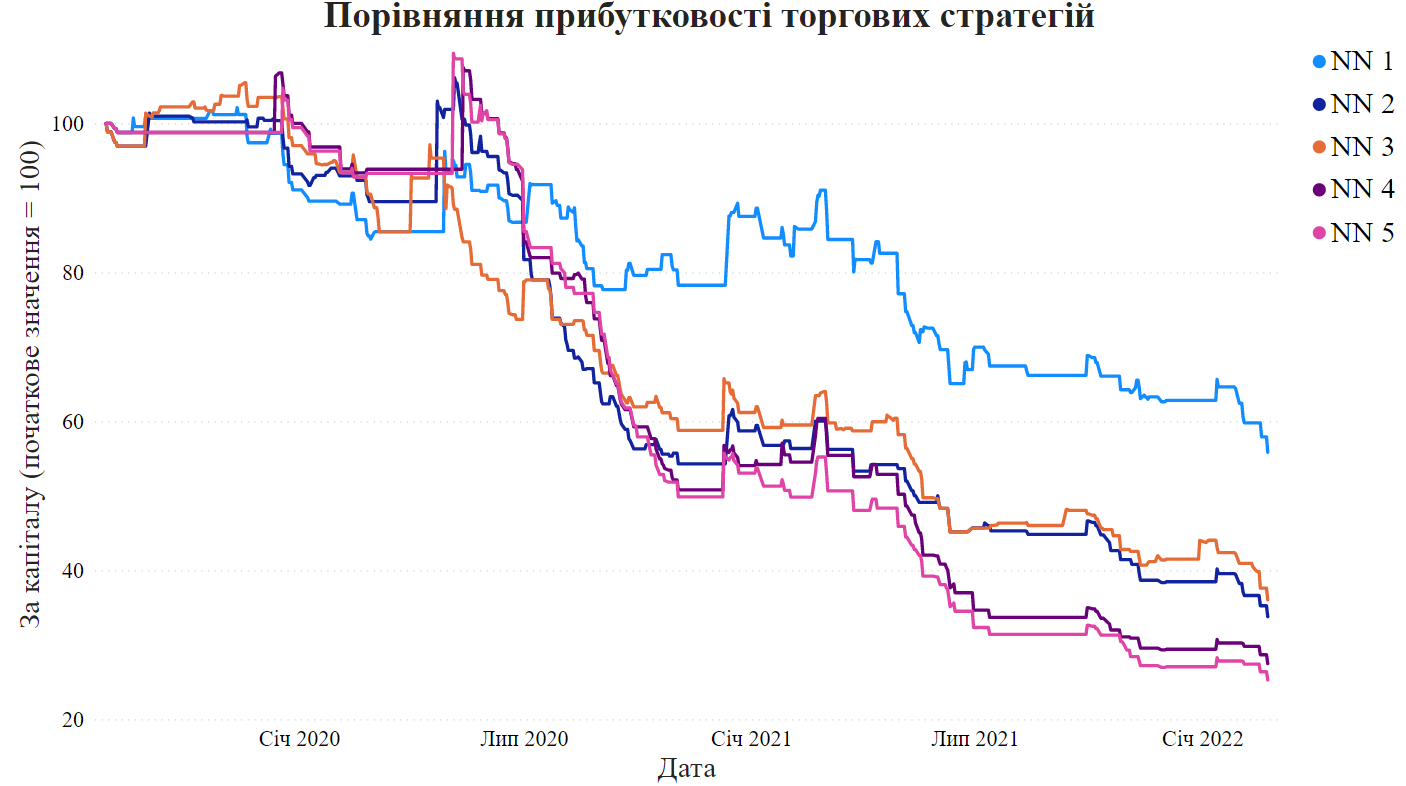
\includegraphics[scale=0.33]{Results Part 3.png}
\end{center}
\end{frame}

\begin{frame}
\frametitle{Результати торгових стратегій, які базуються на прогнозах методів машинного навчання}
\begin{center}
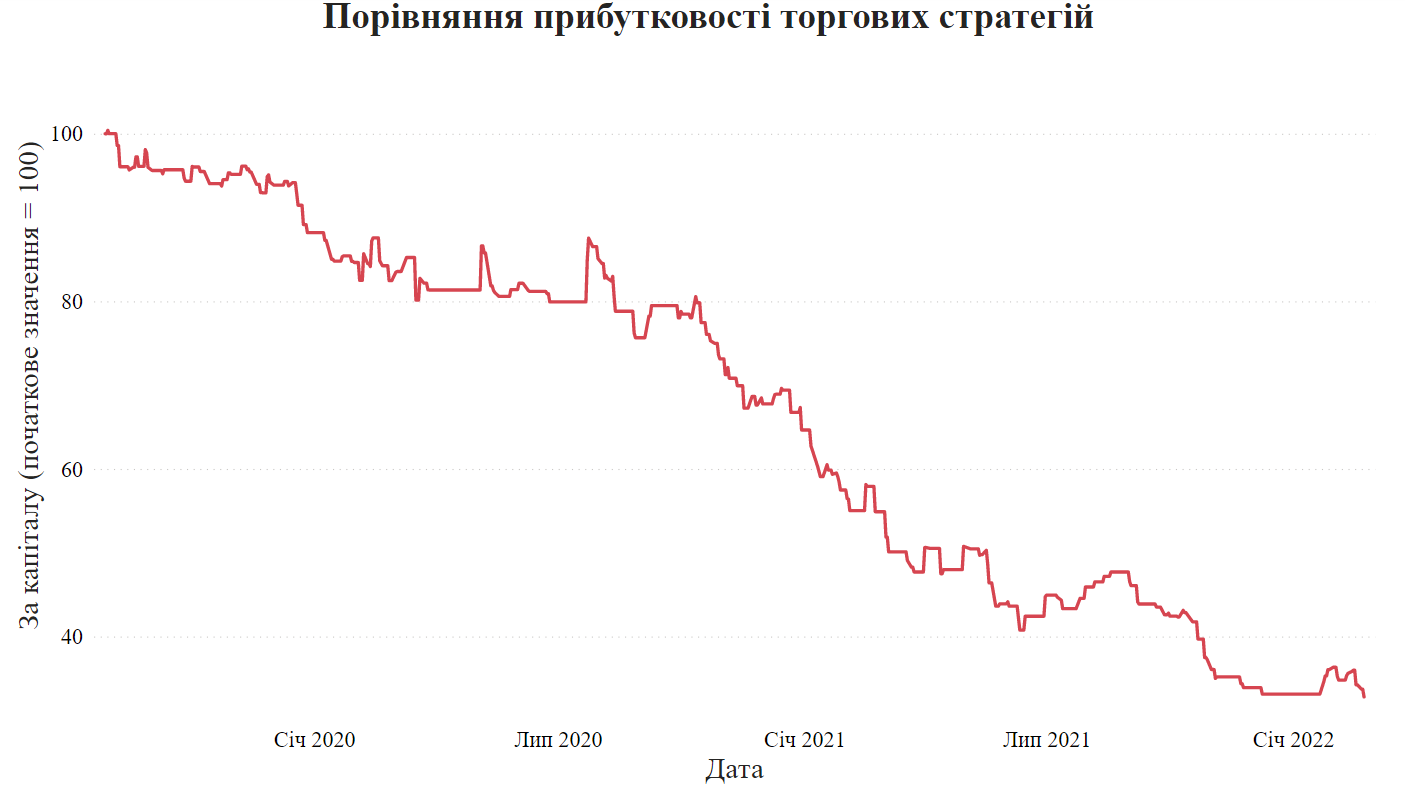
\includegraphics[scale=0.33]{Results Part 4.png}
\end{center}
\end{frame}

\begin{frame}
\frametitle{Результати торгових стратегій, які базуються на прогнозах методів машинного навчання}
\begin{center}
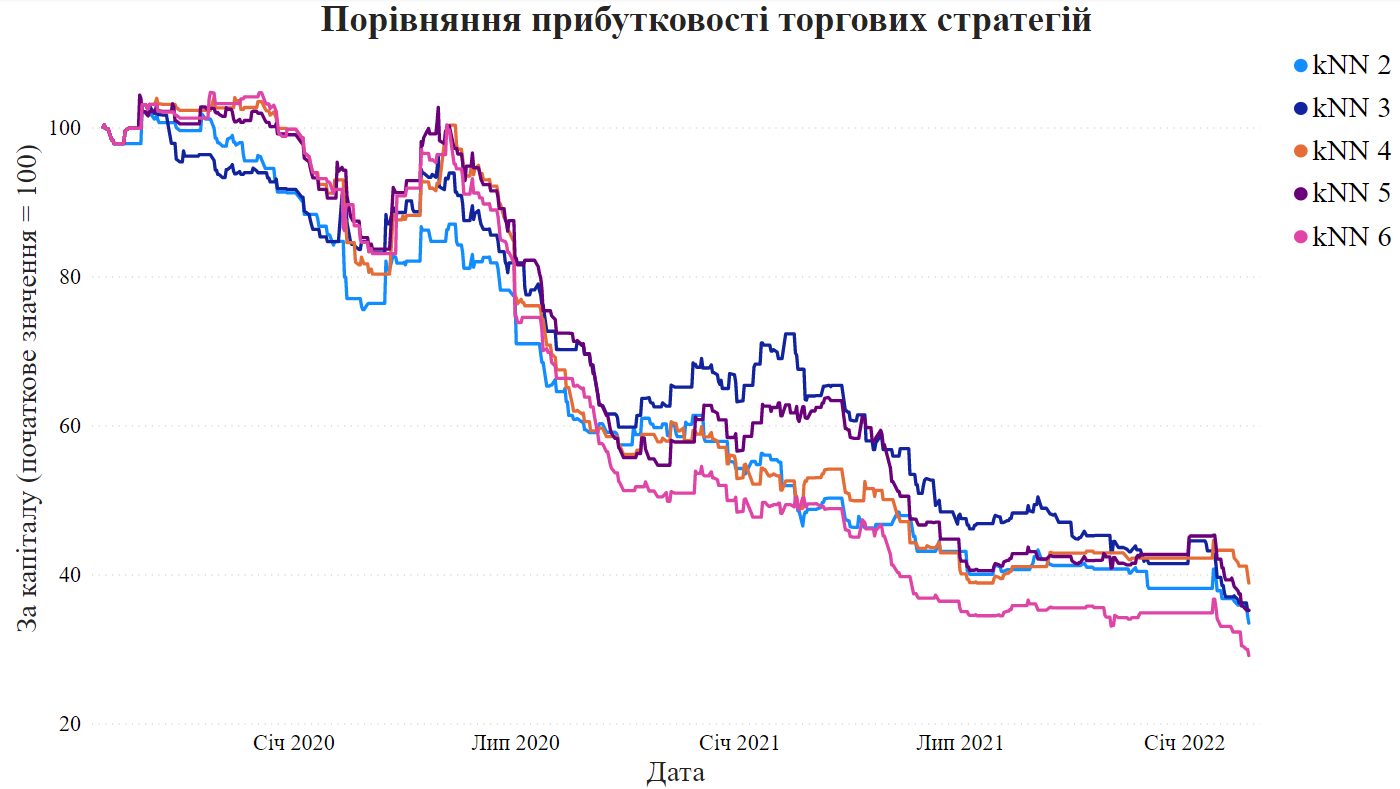
\includegraphics[scale=0.33]{Results Part 5.png}
\end{center}
\end{frame}

\section{Висновки}

\begin{frame}
\frametitle{Висновки}
\begin{itemize}
\item Усі побудовані торгові стратегії, незалежно від того, чи базувалися вони на 
сигналах  методів  технічного  аналізу,  чи  на  прогнозах  моделей  машинного навчання, \alert {\textbf{виявилися збитковими}}; результати наших торгових стратегій програють в порівнянні з пасивною  стратегією  buy-and-hold.  
\bigskip
\item Цей  результат  узгоджується  з  теорією ефективних ринків, яка виключає можливість прибутковості технічного аналізу зокрема та активних інвестиційних стратегій в цілому.
\bigskip
\item Отже, ані використання методів технічного аналізу, ані використання методів машинного навчання \alert {\textbf{не дозволило б нам переграти ринок}} (Для індексу українських акцій UX за період з 2008 по 2022 роки)
\bigskip
\definecolor{cadmiumgreen}{rgb}{0.0, 0.42, 0.24}
\item \textcolor{blue} {У подальшому доцільно було б розглянути} У  подальшому  доцільно  було  б  розглянути  інші  методи  машинного навчання, збільшити кількість індексів, та спробувати замінити сигнали  методів технічного  аналізу  фундаментальними даними
\bigskip
\end{itemize}
\end{frame}

\begin{frame}
\frametitle{Q\&A}
\begin{center}
\bigskip
\textcolor{blue}{\huge Дякую за увагу!} \\
\end{center}
\begin{multicols}{2}

\vbox{\vspace{0.8cm}}
Дані та код для обробки даних, навчання моделей, розрахунків та побудови графіків (.ipynb), а також .pbix файли доступні в репозиторії (github), перейти до якого можна відсканувавши QR-код праворуч.
\columnbreak
\hspace{5mm}
\includegraphics[scale=0.12]{qr-code.png}
\end{multicols}
\end{frame}

\begin{frame}
\frametitle {Прогнозування динаміки Індексу українських акцій (UX) за допомогою методів технічного аналізу та машинного навчання}
\setbeamertemplate{section in toc}[circle]
%\setbeamercolor{section in toc}{fg=UniBlue}
%\setbeamercolor*{section in toc}{fg=UniBlue}
\tableofcontents
\end{frame}

\end{document}
